\documentclass[../revisedMain.tex]{subfiles}
\begin{document}
Unfortunately, there's no simple and easy way to calculate limits. The simplest way is just to ``plug in'' to the function but at some points like holes in the graph or $\infty$, we don't have that luxury. Instead, we can reduce or rewrite equations and also apply some general common sense. For example, $\lim\limits_{x\to\infty} \frac{1}{x}$ must be 0 because as $x$ gets larger, $\frac{1}{x}$ gets smaller to some point at which it must be 0. Using reduction and logic, we may progress on to more complex ideas involving limits where direct substitution fails.
\paragraph{Rules} There are simple rules for limits: $$\lim_{x\to c} f(x)*g(x) = \lim_{x\to c} f(x) * \lim_{x\to c} g(x)$$$$\lim_{x\to c} \frac{f(x)}{g(x)} = \frac{\lim\limits_{x\to c} f(x)}{\lim\limits_{x\to c} g(x)}$$$$\lim_{x\to c} f(x)^n = \left(\lim_{x\to c} f(x)\right)^n$$
The same is true for function addition, subtraction, etc.
\paragraph{``Plugging In''} In the end, all limit problems will need to have their value inserted at some time. For example, the limit $\lim\limits_{x\to 0} x^2+1=1$. No tricks here, plugging in 0 does return 1. We do not have to deal with any division by zero or infinities, so there is no need to manipulate the problem.
\paragraph{Reduction} Reduction is relatively simple. If we go back to our example of $$f(x)=\frac{x^2-4}{x-2}$$ we can see that this problem can factor into $$f(x)=\frac{(x-2)(x+2)}{x-2}$$ which cancels and gives us $$f(x)=x+2$$We now see that there does exist a limit at $x=2$, $f(2)=2+2=4$. Previously, directly plugging in 2 would not return a real value.
\paragraph{Sense at $\infty$} $\infty$ is a hard concept to grasp and work with in mathematics. Limits can make this easier because while we cannot \textit{directly compute} $\infty$, we can approximate it exactly. For example, in the case of $f(x)=\displaystyle\frac{1}{x^2}$, we see that the limit at $\infty$ must be zero. As $x$ increases, $f(x)$ drops ever closer to 0:$$f(10)=0.01$$$$f(100)=0.0001$$$$f(1000)=0.000001$$$$etc.$$ Similarly, as $x$ approaches $\infty$, $$g(x)=\frac{3x}{4x+1}$$ approaches $\frac{3}{4}$: $$g(10)=\frac{30}{41}$$$$g(100)=\frac{300}{401}$$$$g(1000)=\frac{3000}{4001}$$$$etc.$$
\newpage
\subsection{When Limits Don't Exist} Limits don't exist when:
\begin{enumerate}
\item $\lim\limits_{x\to c^+} \neq \lim\limits_{x\to c^-}$
\begin{center}
\begin{tikzpicture}
	\begin{axis}
	\addplot[domain=-1:0,blue,samples=50]{x^2+1};
	\addplot[domain=0:1, blue]{-.25*x+0.75};
	\addplot[holdot] coordinates{(0,1)};
	\addplot[dot] coordinates{(0,.75)};
	\end{axis}
\end{tikzpicture}
$$\lim_{x\to 0} f(x) \text{ Does Not Exist}$$
\end{center} 
\par The reason why the limit cannot exist at 0 here is that when $f(x)$ approaches 0 from the right side ($0^-$), the limit is 1. As $f(x)$ approaches 0 from the left side ($0^+$), the limit is 0.75. The limit is one point and because $0.75\neq 1$, there is no solution.
\newpage
\item The graph oscillates uncontrollably:
\begin{center}
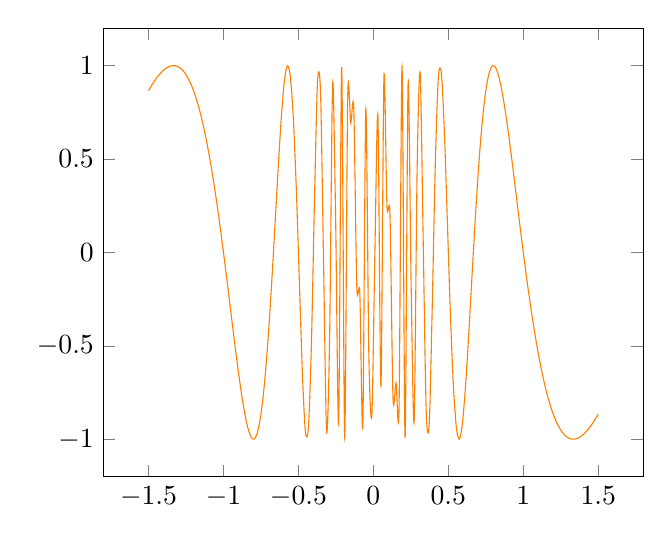
\begin{tikzpicture}
	\begin{axis}
	\addplot[domain=-1.5:1.5,orange,smooth,samples=150]{sin(360*(x)^-1)};
	\end{axis}
\end{tikzpicture}
$$\lim_{x\to 0} \text{sin} \left ( \frac{1}{x} \right ) \text{ Does Not Exist}$$
\end{center} \par The graphing utility doesn't even have any idea what's going on. We can't blame it because the graph starts oscillating faster and faster closer to 0. There is no point the graph can approach. Therefore, the limit must not exist here.
\newpage
\item The graph oscillates at $\infty$
\begin{center}
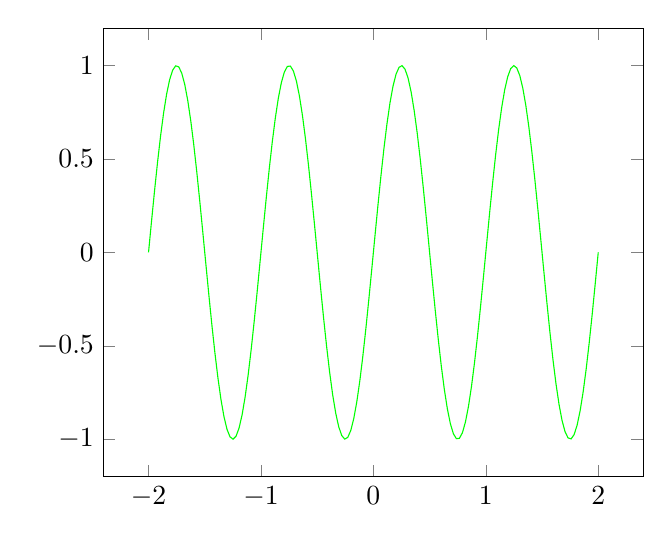
\begin{tikzpicture}
	\begin{axis}
	\addplot[domain=-2:2,green,samples=150]{sin(360*x};
	\end{axis}
\end{tikzpicture}
$$\lim_{x\to\infty} \text{sin}(x) \text{ Does Not Exist}$$
\end{center}
\par Is $\infty$ an integer? Or where does it fall exactly? If you define $\infty$ to be a value, something can always be added to that value. Therefore, there is no single number that this graph will approach. In fact, it will approach all numbers in the interval [-1,1]. For a periodic graph like sin($x$), there can be no limit because the graph will never stop oscillating.
\end{enumerate}
\end{document}